\chapter{Data acquisition and structure}\label{dataacc}
In this chapter we will consider how we can develop a tool that generates and visualizes the layout of network topologies based on constructed, artificial data and real, mined data.
We will have great need for both artificial and real data in chapter \ref{chap:clustering} where we consider algorithms that enables distributed clustering of access points. This chapter also covers the storing of the data in question, how to structure it and visualize it both correcly and meaningfully in a web application. 

\section{Motivation}
The data mining is important as we don't have the time nor the resources to organize a large enough testbed to purposefully evaluate the algorithms and suggestions that we will look at in the 
consecutive chapter. A sufficient testbed would require a large amount of routers (100-200 for a low scale test) in a small geographical area, preferably installed in 
residential apartment buildings. Not only would the creation of such a testbed require a lot of physical equipment, but there is also a lot of logical challenges 
that would have to be overcome, such as communication protocols and distributed consensus. These are problems we will address in chapter \ref{chap:distr}.
While said challenges could be overcome, going directly from a concept idea to a large tesbed without having any empirical indication of which approaches have merit, is 
hardly advisable. Hence we gather data with the motivation of being able to perform realistic calculations and simulations, and with that enhance the believability of the results produced. 

\section{Requirements}
SSID, current channel frequency, radio power, physical data rate and supported 802.11 standards are just a few properties of a single real-life access point.
We are going to represent such access points in our network topology, but the access points we are representing will not be in the transmission (CSMA/CA) state where
most of theese properties are used. Our access points are in a state we can call the \textit{group discovery state}, where the goal is to find or create a group to be a part of
so that a channel can be assigned before transmission happens. Hence, to perform our computations, we don't have to consider many of these properties.
Actually, we will only store each access point's SSID, because this is a practical way to uniquely identify them \footnote{In the real world this is of course not the case,
but we will enforce it in our computations. We could just as well call it a unique id.},  and the the list of other access points that can be seen through a WLAN scan with
and their observed signal strength. These are the only metrics we require, but unfortunately there is no publicly available data source that contains the subjective radio scans
of a large amount of access points in the same area.

As a basis for our simulation we will represent nodes on a two-dimensional grid. Each dataset has to contain a set of nodes with two coordinates $x$ and $y$ so they can
positioned on the grid. When the nodes are placed on the grid they represent a network topology
and it will be possible to compute an estimation of which nodes can hear each other on the radio, and add these to each node's SSID-scan list.
This list contains the names of all the nodes it can hear, and how loud it is heard measured in $-dBi$.
Additionally the following parameters should be variable depending on each test scenario:

\begin{itemize}
	\item Topology size with the possibility to give variable width of x- and y-axis as input arguments. These unit of the axes is meters.
	\item Number of nodes to place on the topology
	\item Minimum distance between nodes (in meters). This is only to avoid unlikely placement and extreme interference of nodes that are placed on top of each other. 
	\item Minimum loudness measured in $-dBi$ for a node to account another node as a neighbour (e.g -100 is too low for anyone to hear).
\end{itemize}


	\section{Program design}\label{prog_design}
	The topology generation program consists of two main functionalitites.

	The first functionality is creating a topology and generate nodes which are uniformly
	and randomly positioned on the network topology. The size of the topology, the number of nodes and the minimum distance
	between nodes are properties that are passed as input arguments to the program.

	The second functionality is performing the calculation of which nodes can actually hear each other over the radio.
	We are assuming all nodes	are transmitting with equal strength, and that the environment is flat and obstacle free. 
	All the neighbouring nodes that can be heard by a node, is added to its list of neighbours, and it stores the $-dBi$ value so it later can be shared with
	the group. The interference levels between access points are calculated by iterating through every access point. For each node $N$ we record its x and y position,
	and then start a second iteration through the nodes. For each node $n$ in the second iteration we calculate the distance $d$ in
	meters between $N$ and $n$ using Euclidean distance. The formula for isotropic antennas is described by Friis \cite{Friis46}, and can be used to
	derive the formula for free space path loss \cite{FSPL} that is as follows:
\[
	FSPL(dB) = 10\log_{10} \left( \frac{ (4 \pi f d)}{c} ^2 \right) 
\]	
	Where $d = distance$, $f = frequency$ and $c=constant$. The constant $c$ is used to account for different units. We will use the meters to denominate the distance,
	and megahertz for the frequency. The resulting formula which will be implemented in the program is
\[
	FSPL(dB) = 20\log_{10}\left( f \right)  + 20\log_{10} \left(d\right) - 27.55
\]	
	As we have to compute the distance from all nodes to every other node, the topology generation program has $O(n^2)$ complexity. A simplified version of the code
	can be seen in figure \ref{fig:dbiCreation}. 

	The resulting program, written in Python 3\cite{Python3}, contains an importable \textit{topology class}. This way, for further testing we can use different data
	sources to get the positions of nodes, and only let the topology class compute the list of neighbours. 
	

	\begin{figure}[H]
		\begin{python}
#In topology class
def measureInterference(self):
 for nodeSubject in self._nodes:  
  for nodeObject in self._nodes:
    nodeSubject.calculateInterferenceTo(nodeObject) 

#In node class
def calculateInterferenceTo(self, nodeObject):
 if self == nodeObject:
  return
 dist = round(self.distanceTo(nodeObject))

#If  nodes have same coordinate, set high interference. 
 if (dist == 0):
  dBi = -40
 else:
  dBi  = self.measureDbi(dist) * -1

def measureDbi(self, dist):
 return (20 * math.log(self._frequency, 10)) + 
(20 * math.log(dist, 10)) - 27.55

			\end{python}
			\caption{Computing the interference between nodes}
			\label{fig:dbiCreation}
			\end{figure}

			\section{Data output and visual representation} \label{simulationrep}
			The result of the topology generation is stored in a JSON\cite{JSON} data file. The data file contains the height and width of the the generated topology, as well
			as the number of nodes. A \verb|nodes| object consists of as many JSON node-objects as there are nodes. Figure \ref{fig:nodeStruct} illustrates the node structure
			and is an example of how a node with two neighbours will look.
			\begin{figure}[H]
			\begin{minipage}{\linewidth}
			\begin{lstlisting}[language=json]
{
  "mapWidth": 100,
  "mapHeight": 100,
  "nodeCount": 3,
  "nodes": {
    1: {
    "posX": 50,
    "posY": 50, 
    "ssid": "NODE1", 
    "neighbourCount": 2, 
    "neighbours": {
      0: {
        "ssid": NODE2,
        "dbi": -77.23
        },
      1: {
        "ssid": NODE3,
        "dbi": -79.52
        }
      }
    }
  },
...
}
\end{lstlisting}
\end{minipage}
\caption{JSON output structure}
\label{fig:nodeStruct}

\end{figure}
The program can be run in the following way
\begin{verbatim}./GenerateTopology.py -n 500 -w 100 -h 100 --space 10 --dbi 85 \end{verbatim}
Which instructs the program to create a topology with 500 nodes. The topology should be 100 by 100 meters large, and there should be at least 10 meters
between each node. The $dbi$ parameter makes sure that only nodes which can be heard with a $-dBi$-value of $-85$ or larger should appear in the neighbour list. 
The output from this specific run is a 23.2 MB large file containing the resulting topology-data in JSON.

By writing a simple HTML and JavaScript browser application, we can parse the JSON and visually represent the nodes on a grid.
The result will look like what can be seen in figure \ref{fig:randtop}

\begin{figure}[h]
\center
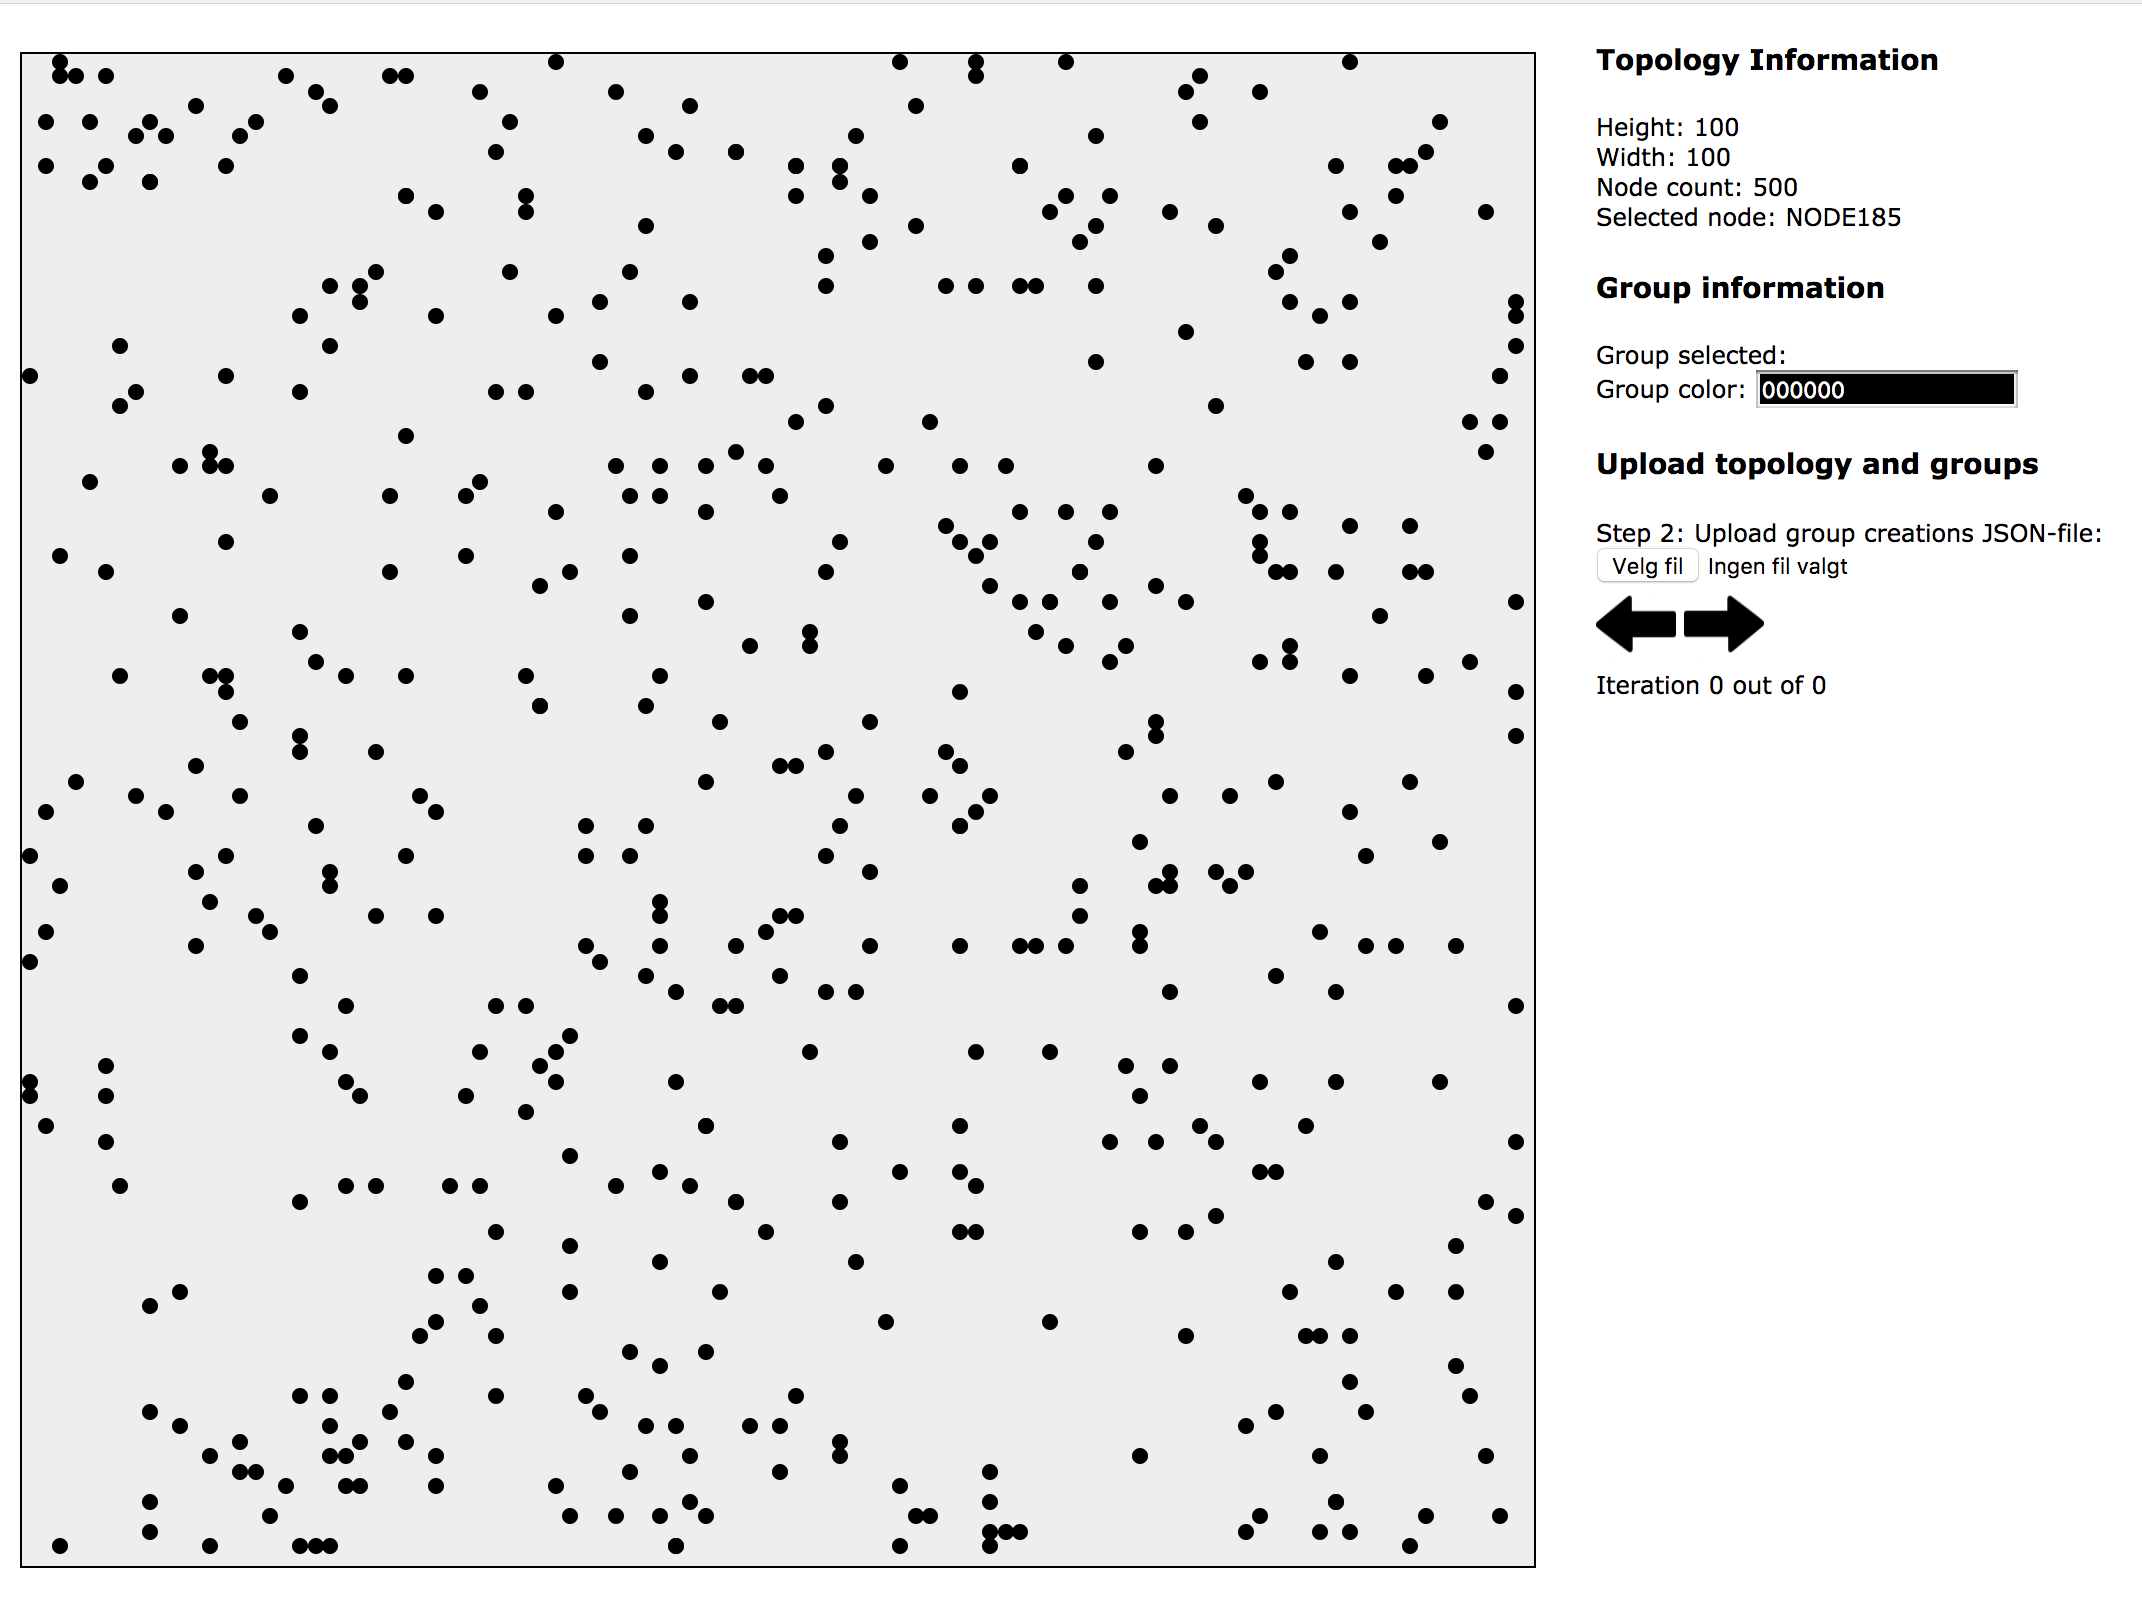
\includegraphics[scale=0.35]{Images/interface.png}
\caption{Generated topology with random, uniform distribution and the interface for viewing topologies}
\label{fig:randtop}
\end{figure}

\section{WiGLE}
WiGLE (Wireless Geographical Logging Engine) \cite{wigle} is a project started in 2001 which purpose is to gather information about wireless networks. All the information
they collect is user submitted stored in their database. Anyone can download an Android app developed and published by WiGLE, and use the app for wardriving,
\footnote{Wardriving is the act of tracking wireless networks using a laptop or a phone,	and then store the information about each network.},
	then submit the data to WiGLE's centralized database. The APs discovered can be viewed on an interactive map provided on WiGLE's website. 
	All the data can also be accessed through a public API which is especially interesting for us. Using their service is entirely free, but the
	amount of data that can be requested is throttled on a day-to-day basis. In the FAQ section on the website its written that the project openly supports research projects, 
	so after contacting them they upgraded the account we will be using for the data requests to a higher daily data quota.

	As the physical location of each access point is estimated using weighted-centroid trilateration, 
	we can fetch the estimated position of each access point. However, the location data is not necessarily always accurate: if the measurements of an access point signal
	strength is done in multiple places (in a way that a line between the measurement locations surrounds the access point), the access point location becomes very precise. 
	On the other hand, if the measurements are taken on only one side of the access point, the measurements are heavily shifted towards that side. {{figure?}} 
	
	Even though the data is not perfect, it is more suited to impersonate the layout of real-life network topologies and give us a better understanding of how what access point
	clustering would look like in real-life. 



	\subsection{REST API}
	WiGLE has a REST API that can be used to retrieve information from their database. The API responds to requests with JSON data. It gives access to a
	number of services such as user profile management, large-scale statistical information about the collected data
	and more specific network searches. An interactive guide to the public API is available at \cite{WigleAPI}. 

	We are going to mine data for the topology generation program, hence the network search service is all we are interested in. There are several ways an access point can be retrieved using
	the network search. We can query specific SSIDs, a range of coordinates, only APs with a minimum signal level, or only query networks that are free to use. As 
	we are only rebuilding the network topology to fit our tailored data structure, we will consider all access points and not filter on any parameters except for coordinates.
	By issuing an API a request for nodes between two latitudes and two longitudes, the response is an array with AP objects within that area.  
	A request will look something like what can be seen in figure \ref{fig:wigReq}.
	\begin{figure}
	\scriptsize
	\begin{lstlisting}[breaklines]
	 https://api.wigle.net/api/v2/network/search?first=0&latrange1=37.80846&latrange2=37.7467&longrange1=-122.5392&longrange2=-122.3813&start=0
	\end{lstlisting}
	\caption{Example of a Wigle API request}
	\label{fig:wigReq}
	\end{figure}

	The parameters $latrange1$ and $longrange1$ are the coordinates that marks the beginning of the area we are interested in and $latrange2$ and $longrange2$ marks the end. 
	We want information about the position of all access points within this range, however WiGLE returns at most 100 results per query. If there are more than 100 access points, we need to change the $start$
	parameter. This parameter tells WiGLE at which offset we want to begin fetching data from. For instance a start value of $0$ means we fetch the first 100 access points, with indexes 0-99. A value of $100$ means that
	we fetch the next 100 APs in the range $100-199$ and so on. The JSON response for a succesful request for one AP can be seen in figure \ref{fig:wigle}. 

	\begin{figure}[h]

	\begin{lstlisting}[language=json]
{
\subsection{Graph history}
	"userfound": false,
	"qos": 0,
	"comment": null,
	"lastupdt": "2015-12-22T17:49:34.000Z",
	"bcninterval": 0,
	"dhcp": "?",
	"lasttime": "2015-12-22T17:49:15.000Z",
	"trilong": 10.82792618,
	"netid": "5C:9E:FF:2B:54:84",
	"freenet": "?",
	"trilat": 62.2816925,
	"name": null,
	"firsttime": "2015-12-22T20:55:01.000Z",
	"type": "infra",
	"ssid": "NETGEAR23",
	"paynet": "?",
	"wep": "2",
	"transid": "20151222-00207",
	"channel": 52
}

\end{lstlisting}
\caption{REST API response with AP data}
\label{fig:wigle}
\end{figure}

The JSON-object in the response contains quite a lot of information about all of the APs retrieved. We wont be using most of this data, but it is worth noting that some of it could be used to perfect the search. For instance the last updated parameter could
be a way to refine the access points retrieval, so that access points that has been long gone is not taken into consideration. The most valueable properties for us is $trilong$ and $trilat$. As the names suggest these contain the position calculated
by the weighted-centroid triliteration. 

\subsection{The Haversine Formula}
As seen in the previous section, WiGLE provides data about the location of access points and a way for us to retrieve this data in a usable format. 
At this point we could create a program that operates directly on the longitudes and latitudes retrieved.
This program would also need to be able to use the FPSL formula on global coordinates to compute the radio scans of each AP,
and to properly visualize the data we would have to reinstall the nodes on a globe. This implementation requires a lot of extra labour, and seems especially
redundant when we already have a working program that already has the aforementioned functionality.
The problem is that our previous work relies on a two dimensional Cartesian coordinate system.
To be able to reuse what we have have already built, the geographic coordinates has to be translated into coordinates in Euclidean space.

The haversine formula \cite{virtues} is used to accurately compute the great-circle distance between two global coordinates.

\[
	d =2R sin^{-1} \left(\sqrt{ \left(sin\left(\frac{\varphi_2-\varphi_1}{2} \right)\right)^2 + cos(\varphi_1) * cos(\varphi_2) * sin\left(\left( \frac{\lambda_2 - \lambda_1}{2} \right)\right)^2} \right)
	%a = sin²(Δφ/2) + cos φ1 ⋅ cos φ2 ⋅ sin²(Δλ/2)
	%FSPL(dB) = 20\log_{10}\left( f \right)  + 20\log_{10} \left(d\right) - 27.55
\]	

Where $d$ is the distance between two latitudes $\varphi_1$ and $\varphi_2$ and two longitudes $\lambda_1$ and $\lambda_2$. $R$ is the radius of the
sphere, which in this context is the earth's radius. 

This can also be expressed with a two-parameter inverse tangent function \cite{chamberlain_2017}, as long as neither of the
parameters are zero. 

\begin{flalign}
	\nonumber a &= \left(sin\left(\frac{\varphi_2-\varphi_1}{2} \right)\right)^2 + cos(\varphi_1) * cos(\varphi_2) * sin\left(\left( \frac{\lambda_2 - \lambda_1}{2} \right)\right)^2 \\
	\nonumber c &= 2*atan2(\sqrt{a}, \sqrt{(1-a)}) \\
	\nonumber d &= c * R
	%a = sin²(Δφ/2) + cos φ1 ⋅ cos φ2 ⋅ sin²(Δλ/2
	%FSPL(dB) = 20\log_{10}\left( f \right)  + 20\log_{10} \left(d\right) - 27.55
\end{flalign}


The python implementation of the formula can be seen in figure \ref{fig:haversine}. It is imortant to note that the degrees taken as input
has to been converted to radians before inserting it in the formula. 

	\begin{figure}[H]
		\tiny
		\begin{python}
def distanceBetweenCoordinates(lat1, lat2, long1, long2):
	deltaLon = math.radians(long2 - long1)
	deltaLat = math.radians(lat2 - lat1)
	a = (math.sin(deltaLat / 2))**2 + math.cos(math.radians(lat1)) * math.cos(math.radians(lat2)) * (math.sin(deltaLon/2))**2
	c = 2 * math.atan2(math.sqrt(a), math.sqrt(1 - a)) 
	R = 6371000
	d = round(c * R)
	return d
	\end{python}
			\caption{Implementation of haversine distance}
			\label{fig:haversine}
	\end{figure}


This can be used to get the distance in meters between the boundaries of our area of interest. When the data is retrieved from
WiGLE we can use the specified coordinates to compute the size of the cartesian coordinate system.
The distance between the first latitude $\varphi_{start}$ and the second latitude $\varphi_{stop}$
is calculated. This is done by using the same longitude  $\lambda_1 = \lambda_2$, and returns the size of the x-axis in meters.
The opposite has to be done to get the size of the y-axis, using $\lambda_{start}$ and $\lambda_{stop}$ and equal longitudes.
The same approach can be used to place each node on the coordinate system, where the first set of the coordinates is
$\varphi_{start}$ and $\lambda_{start}$, and the second set is the coordinates of the AP.
\subsection{Data output}
The resulting python program \ref{appendix:wigleprogram}takes an output filename and two latitudes and two longitudes as input. It queries WiGLE's API for all the APs between these coordinates.
As long as the number of APs in the coordinate range does not exceed the daily data limit, all the data will be stored in a topology datastructure imported 
from the topology generation program in section \ref{prog_design}. The APs will be placed correctly relative to each other, with real world distance between them,
based on the coordinates of each AP. 

{{wigle data figure, overlaid map}}

